\documentclass[12pt]{article}
\usepackage[english]{babel}
\usepackage{natbib}
\usepackage{url}
\usepackage[utf8x]{inputenc}
\usepackage{amsmath}
\usepackage{graphicx}
\graphicspath{{../docs/img/}}
\usepackage{parskip}
\usepackage{fancyhdr}
\usepackage{vmargin}
\usepackage{xcolor}
\usepackage{booktabs}
\usepackage{float}
\usepackage{pgfplots}
\usepackage{tikz}
\pgfplotsset{width=10cm,compat=1.9}

\setmarginsrb{3 cm}{2.5 cm}{3 cm}{2.5 cm}{1 cm}{1.5 cm}{1 cm}{1.5 cm}

\title{Sprint 4 Backlog}								% Title
\author{Thierry's Minions}								% Author
\date{12 Nov 2018}											% Date

\makeatletter
\let\thetitle\@title
\let\theauthor\@author
\let\thedate\@date
\makeatother

\pagestyle{fancy}
\fancyhf{}
\rhead{\theauthor}
\lhead{\thetitle}
\cfoot{\thepage}

\newcommand*{\userstory}[5][.25em]{
%  \begin{tabular*}{\maincolumnwidth}{l@{\extracolsep{\fill}}r}%
%    {\bfseries #2} & {\bfseries #4}\\%
%    {#3}\\%
%  \end{tabular*}%
%  \ifx&#5&%
%  \else{\\%
%    \begin{minipage}{\maincolumnwidth}%
%      #5%
%    \end{minipage}}\fi%
%  \par\addvspace{#1}
\textbf{#1} 
  }

\newcommand{\roundpic}[4][]{
  \tikz\node [circle, minimum width = #2,
    path picture = {
      \node [#1] at (path picture bounding box.center) {
        \includegraphics[width=#3]{#4}};
    }] {};}

\begin{document}

%%%%%%%%%%%%%%%%%%%%%%%%%%%%%%%%%%%%%%%%%%%%%%%%%%%%%%%%%%%%%%%%%%%%%%%%%%%%%%%%%%%%%%%%%

\begin{titlepage}
	\centering
    \vspace*{0.5 cm}
\roundpic[]{9cm}{9cm}{leader.jpg}

    \textsc{\LARGE Thierry's Minions/Team25\\[0.5em] Deliverable 5}\\[2.0 cm]	
	\textsc{\Large CSCC01 Fall 2018}\\[0.5 cm]				% Course Code
	\rule{\linewidth}{0.2 mm} \\[0.4 cm]
	{ \huge \bfseries \thetitle}\\
	\rule{\linewidth}{0.2 mm} \\[1.5 cm]
	
	\begin{minipage}{0.4\textwidth}
		\begin{flushleft} \large
			\emph{Submitted To:}\\
			Saba Kiaei\\
            Teaching Assistant\\
            Computer Science Department\\
			\end{flushleft}
			\end{minipage}~
			\begin{minipage}{0.4\textwidth}
            
			\begin{flushright} \large
			\emph{Submitted By :} \\
			Rishabh Kaant Sharma\\
            Joseph Sokolon\\
            Balaji Badu\\
            Jayden Arquelada\\
            Edgar Sarkisian\\
		\end{flushright}
        
	\end{minipage}\\[2 cm]
	
	
    
    
    
    
	
\end{titlepage}

%%%%%%%%%%%%%%%%%%%%%%%%%%%%%%%%%%%%%%%%%%%%%%%%%%%%%%%%%%%%%%%%%%%%%%%%%%%%%%%%%%%%%%%%%

\textcolor{black}{\tableofcontents}
\pagebreak

%%%%%%%%%%%%%%%%%%%%%%%%%%%%%%%%%%%%%%%%%%%%%%%%%%%%%%%%%%%%%%%%%%%%%%%%%%%%%%%%%%%%%%%%%

\section{Sprint Tasks}

\subsection{Task 5E: Generate Pie Chart for Report.}
\begin{itemize}%
\item Story Points: 5
\item This task has a dependency on task 5D
\item Generate a PIE Chart from data recieved from server.
\item Add the Chart to the PDF.
\end{itemize}

\subsection{Task 5F: Generate Pie Chart for Report.}
\begin{itemize}%
\item Story Points: 2
\item This task has a dependency on task 5D
\item Generate a Bar Chart from data recieved from server.
\item Add the Chart to the PDF.
\end{itemize}

\subsection{Task 5G: Generate Mock Data to Test Reporting.}
\begin{itemize}%
\item Story Points: 1
\item Fill in templates with mock data so we have a sizable quantitiy of data to display in the reports.
\end{itemize}

\subsection{Task 5H: Integrate and test feature.}
\begin{itemize}%
\item Story Points: 3
\item This task has a dependency on all previous tasks.
\item Ensure the integration between the server and client is working.
\item Test the entire feature and ensure it passes the conditions of acceptance.
\end{itemize}

\subsection{Task 6A: Add template data to the database.}
\begin{itemize}%
\item Story Points: 2
\item Create a collection in database that contains information about all the available templates and their columns.
\end{itemize}

\subsection{Task 6B: Create a GET endpoint which returns names of all the templates.}
\begin{itemize}%
\item Story Points: 3
\item Create a  GET endpoint which returns names of all the templates.
\item Names of templates should come from the TEMPLATES collection.
\end{itemize}

\subsection{Task 6C: Create a GET endpoint which returns all the columns in a specific template.}
\begin{itemize}%
\item Story Points: 5
\item Template should be specified  in the header of request, with key template\_name.
\item Create a GET endpoint which returns all the columns in a specific template.
\item Data of columns should come from the TEMPLATES collection.
\end{itemize}

\subsection{Task 6D: Create new UI for the mid-level query page.}
\begin{itemize}%
\item Story Points: 3
\item Page should allow users to select a template name, column name and generate the report by clicking a button.
\item Don't have to write the controllers as part of this task. Next task handles that.
\end{itemize}

\subsection{Task 6E: Create controllers for the mid-level query page.}
\begin{itemize}%
\item Story Points: 3
\item Create controllers which make requests to the server to populate dropdowns with template and column names.
\item Controller to make request to server to generate data for report is already created. 
\end{itemize}

\subsection{Task 6F: Integrate and test feature.}
\begin{itemize}%
\item Story Points: 2
\item This task has a dependency on all previous tasks.
\item Ensure the integration between the server and client is working.
\item Test the entire feature and ensure it passes the conditions of acceptance.
\end{itemize}

\newpage
\section{Sprint Plan}

\textbf{Sprint 5 : November 10th - November 16th (Saturday - Friday)}
\begin{table}[H]
\begin{tabular}{@{}c|c|c|c|ccccccc@{}}
\toprule
Story & Task & Dependency & \begin{tabular}[c]{@{}c@{}}Story\\ Points\end{tabular} & \begin{tabular}[c]{@{}c@{}}Day\\ 1\end{tabular} & \begin{tabular}[c]{@{}c@{}}Day\\ 2\end{tabular} & \begin{tabular}[c]{@{}c@{}}Day \\ 3\end{tabular} & \begin{tabular}[c]{@{}c@{}}Day \\ 4\end{tabular} & \begin{tabular}[c]{@{}c@{}}Day \\ 5\end{tabular} & \begin{tabular}[c]{@{}c@{}}Day \\ 6\end{tabular} & \begin{tabular}[c]{@{}c@{}}Day \\ 7\end{tabular} \\ \midrule
5     & E    &            & 5                                                      &                                                 &                                                 & JS:5                                             &                                                  &                                                  &                                                  &                                                  \\
5     & F    &            & 5                                                      &                                                 &                                                 & JS:5                                             &                                                  &                                                  &                                                  &                                                  \\
5     & G    &            & 1                                                      &                                                 &                                                 &                                                  & ES:1                                             &                                                  &                                                  &                                                  \\
5     & H    & All        & 3                                                      &                                                 &                                                 &                                                  & JA:3                                             &                                                  &                                                  &                                                  \\
6     & A    &            & 2                                                      &                                                 &                                                 & JS:2                                             &                                                  &                                                  &                                                  &                                                  \\
6     & B    &            & 3                                                      &                                                 &                                                 &                                                  &                                                  & ES:3                                             &                                                  &                                                  \\ 
6     & C    &            & 5                                                      &                                                 &                                                 &                                                  &                                                  & BB:2                                             & BB:3                                             &                                                  \\ 
6     & D    &            & 3                                                      &                                                 &                                                 &                                                  & RS:3                                             &                                                  &                                                  &                                                  \\ 
6     & E    &            & 3                                                      &                                                 &                                                 &                                                  &                                                  & JA:3                                             &                                                  &                                                  \\ 
6     & F    & ALL        & 2                                                      &                                                 &                                                 &                                                  &                                                  &                                                  &                                                  & JS:2                                             \\ \bottomrule
\end{tabular}
\end{table}

\begin{itemize}%
\item Estimated story points team can complete: 32
\item The team believes they can complete User Story 5 by end of day 4, \& User Story 6 by end of the day 7. 
\end{itemize}

\newpage

\section{Sprint Report}

\textbf{Sprint 5 : November 10th - November 16th (Saturday - Friday)}
\begin{table}[H]
\begin{tabular}{@{}c|c|c|c|ccccccc@{}}
\toprule
Story & Task & Dependency & \begin{tabular}[c]{@{}c@{}}Story\\ Points\end{tabular} & \begin{tabular}[c]{@{}c@{}}Day\\ 1\end{tabular} & \begin{tabular}[c]{@{}c@{}}Day\\ 2\end{tabular} & \begin{tabular}[c]{@{}c@{}}Day \\ 3\end{tabular} & \begin{tabular}[c]{@{}c@{}}Day \\ 4\end{tabular} & \begin{tabular}[c]{@{}c@{}}Day \\ 5\end{tabular} & \begin{tabular}[c]{@{}c@{}}Day \\ 6\end{tabular} & \begin{tabular}[c]{@{}c@{}}Day \\ 7\end{tabular} \\ \midrule
5     & E    &            & 5                                                      &                                                 &                                                 & RS:2                                             & RS:3                                             &                                                  &                                                  &                                                  \\
5     & F    &            & 5                                                      &                                                 &                                                 &                                                  & RS:5                                             &                                                  &                                                  &                                                  \\
5     & G    &            & 1                                                      &                                                 &                                                 &                                                  &                                                  &                                                  &                                                  &  ES:3                                            \\
5     & H    & All        & 3                                                      &                                                 &                                                 &                                                  &                                                  & JA:3                                             &                                                  &                                                  \\
6     & A    &            & 2                                                      &                                                 &                                                 & JS:2                                             &                                                  &                                                  &                                                  &                                                  \\
6     & B    &            & 3                                                      &                                                 &                                                 &                                                  &                                                  &                                                  & ES:3                                             &                                                  \\ 
6     & C    &            & 5                                                      &                                                 &                                                 &                                                  &                                                  & BB:2                                             & BB:3                                             &                                                  \\ 
6     & D    &            & 3                                                      &                                                 &                                                 &                                                  &                                                  &                                                  &                                                  & RS:3                                             \\ 
6     & E    &            & 3                                                      &                                                 &                                                 &                                                  &                                                  & JA:3                                             &                                                  &                                                  \\ 
6     & F    & ALL        & 2                                                      &                                                 &                                                 &                                                  &                                                  &                                                  &                                                  &                                                  \\ \bottomrule
\end{tabular}
\end{table}

\begin{itemize}%
\item Actual story points burned: 21
\item Rishabh took tasks 5E and 5F from Joey.
\item Balaji worked on, but didn't complete task 6C, The task will be carried over to next sprint.
\item Joey didn't complete task 6F, The task will be carried over to next sprint.
\item Story 6 - Mid Level Report Generation will be carried over to next sprint.
\item The team completed User Story 5 on day 5 of the sprint. 
\end{itemize}

\section{Sprint Burndown Chart}

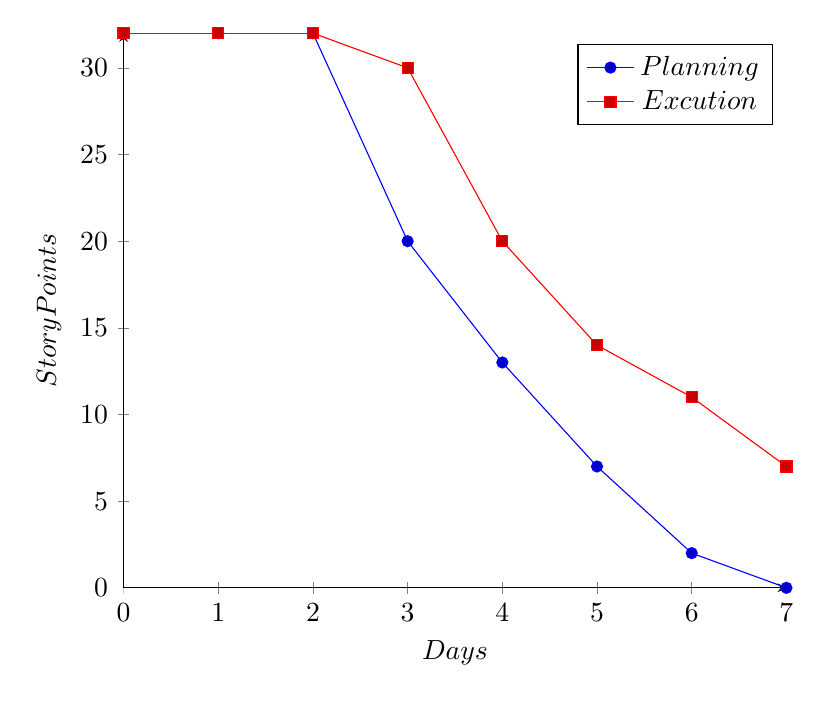
\begin{tikzpicture}
\begin{axis}[
    axis lines = left,
    xlabel = $Days$,
    ylabel = {$Story Points$},
]
\addplot coordinates {(0,32) (1,32) (2,32) (3,20) (4,13) (5,7) (6,2) (7,0)};
\addlegendentry{$Planning$}
\addplot coordinates {(0,32) (1,32) (2,32) (3,30) (4,20) (5,14) (6,11) (7,7)};
\addlegendentry{$Excution$}
\end{axis}
\end{tikzpicture}

\newpage
\bibliographystyle{plain}
\bibliography{biblist}

\end{document}